\documentclass[graphics]{beamer}

\usepackage{graphicx}
\usepackage{verbatim}
\usepackage{wrapfig}
\useoutertheme{shadow}
%\usecolortheme{orchid}
\usecolortheme{seahorse}


% math commands
\newcommand{\be}{\begin{eqnarray}}
\newcommand{\ee}{\end{eqnarray}}
\newcommand{\beq}{\begin{equation}}
\newcommand{\eeq}{\end{equation}}
\def\simless{\mathbin{\lower 3pt\hbox
      {$\rlap{\raise 5pt\hbox{$\char'074$}}\mathchar"7218$}}}
\def\simgreat{\mathbin{\lower 3pt\hbox
      {$\rlap{\raise 5pt\hbox{$\char'076$}}\mathchar"7218$}}} %> or of order

% variables

\def\toonscale{0.45}
\def\mboxy#1{\mbox{\small #1}}


\begin{comment}
\AtBeginSection[]{
  \frame{
    \frametitle{Outline}
    \tableofcontents[currentsection]
  }
}
\end{comment}

\title{CITA: A Pillar of the Canadian Astronomical Community
}
\subtitle{}
\author[U. Pen]{Ue-Li Pen
\\[8mm] 
}
\date{May 26, 2018}

% abstract: 
%I will review the history of CITA, and potential scenarios for the future.   
%Synergy with the Canadian and global community have been the
%hallmark, with adaptive catalytic roles in HPC, new funding, HQP and beyond.


\begin{document}


\begin{comment}
  \subsection{Outline}

  \frame{
    \frametitle{Outline}
    \tableofcontents
  }
\end{comment}



\frame{\maketitle}



  \frame{
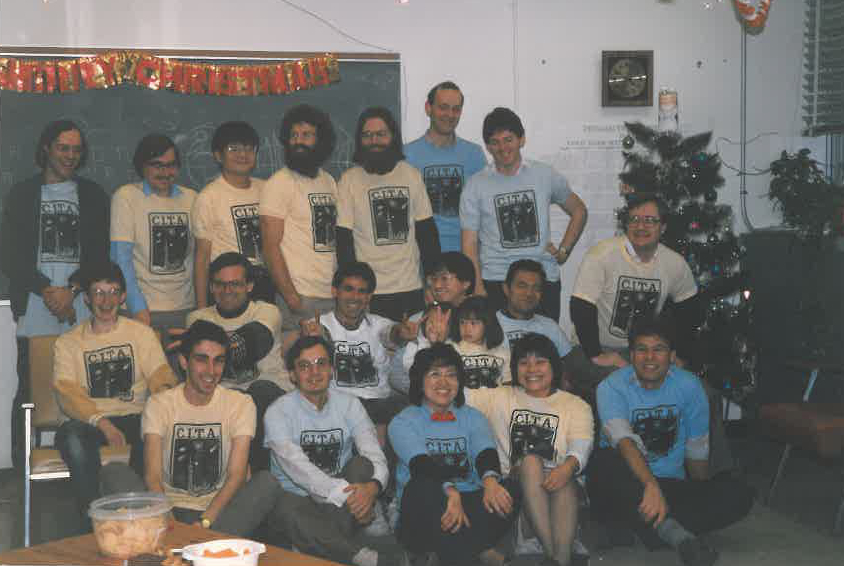
\includegraphics[width=4.2in]{Figures/CITA_many_yrsAgo.jpg}
  }

  \frame{
\includegraphics[width=4.2in]{Figures/bondfest.jpg}
  }


 \frame{
\vspace{-0.5in}
    \frametitle{Mission}
    \begin{itemize}
    \item foster interactions in theory across Canada
    \item world leading theoretical astrophysics research 'branding',
      strong alumni grouping
    \item create national opportunities: national fellows, Canada fellows
    \item generate new funding streams
    \item complementary to NRC, Perimeter Institute
    \end{itemize}
  }

  \frame{
\vspace{-0.5in}
    \frametitle{Snapshot}
    \begin{itemize}
      \item 13+14th floor of Toronto physics building
      \item 6 faculty
      \item 4 staff, 23 postdocs, 22 graduate students
      \item small 'sunnyvale' computer cluster available to national astro
        community
    \end{itemize}
  }

  \frame{
    \frametitle{History}
    \begin{itemize}
      \item established in 1985, first members Dick Henrickson+Peter Martin
      \item fills several niches:
      \item world leading theoretical astrophysics institute
      \item supports Canadian theory: attract+retain HQP, over 20
        CITAzens in faculty positions in Canada, +NF,GS, over 130 worldwide
      \item leadership in Canadian HPC: from SUN, SGI to McKenzie
        (top500 record in Canada), Niagara, Sunnyvale
      \item draw new funding into astrophysics: CERC, SOSCIP, ORF-RE, OCE, RPP
    \end{itemize}
}


  \frame{
%\vspace{-0.5in}
    \frametitle{Industrial Bridges}
    \begin{itemize}
        \item AMD Markham labs (formerly ATI):  MHD software collaboration
        \item joint development of 7 PFLOP (FP32) CHIME 512 GPU
          correlator: low precision fixed point DSP (Vanderlinde et al)
        \item Dark Energy and FRB hardware and software of direct application to
          machine learning
        \item SOSCIP, IBM, Thoth, Skywatch ++: HQP support, FPGA platforms, BGQ, GPU, etc 
    \end{itemize}
\vspace{-0.01in}\hspace{.3in}
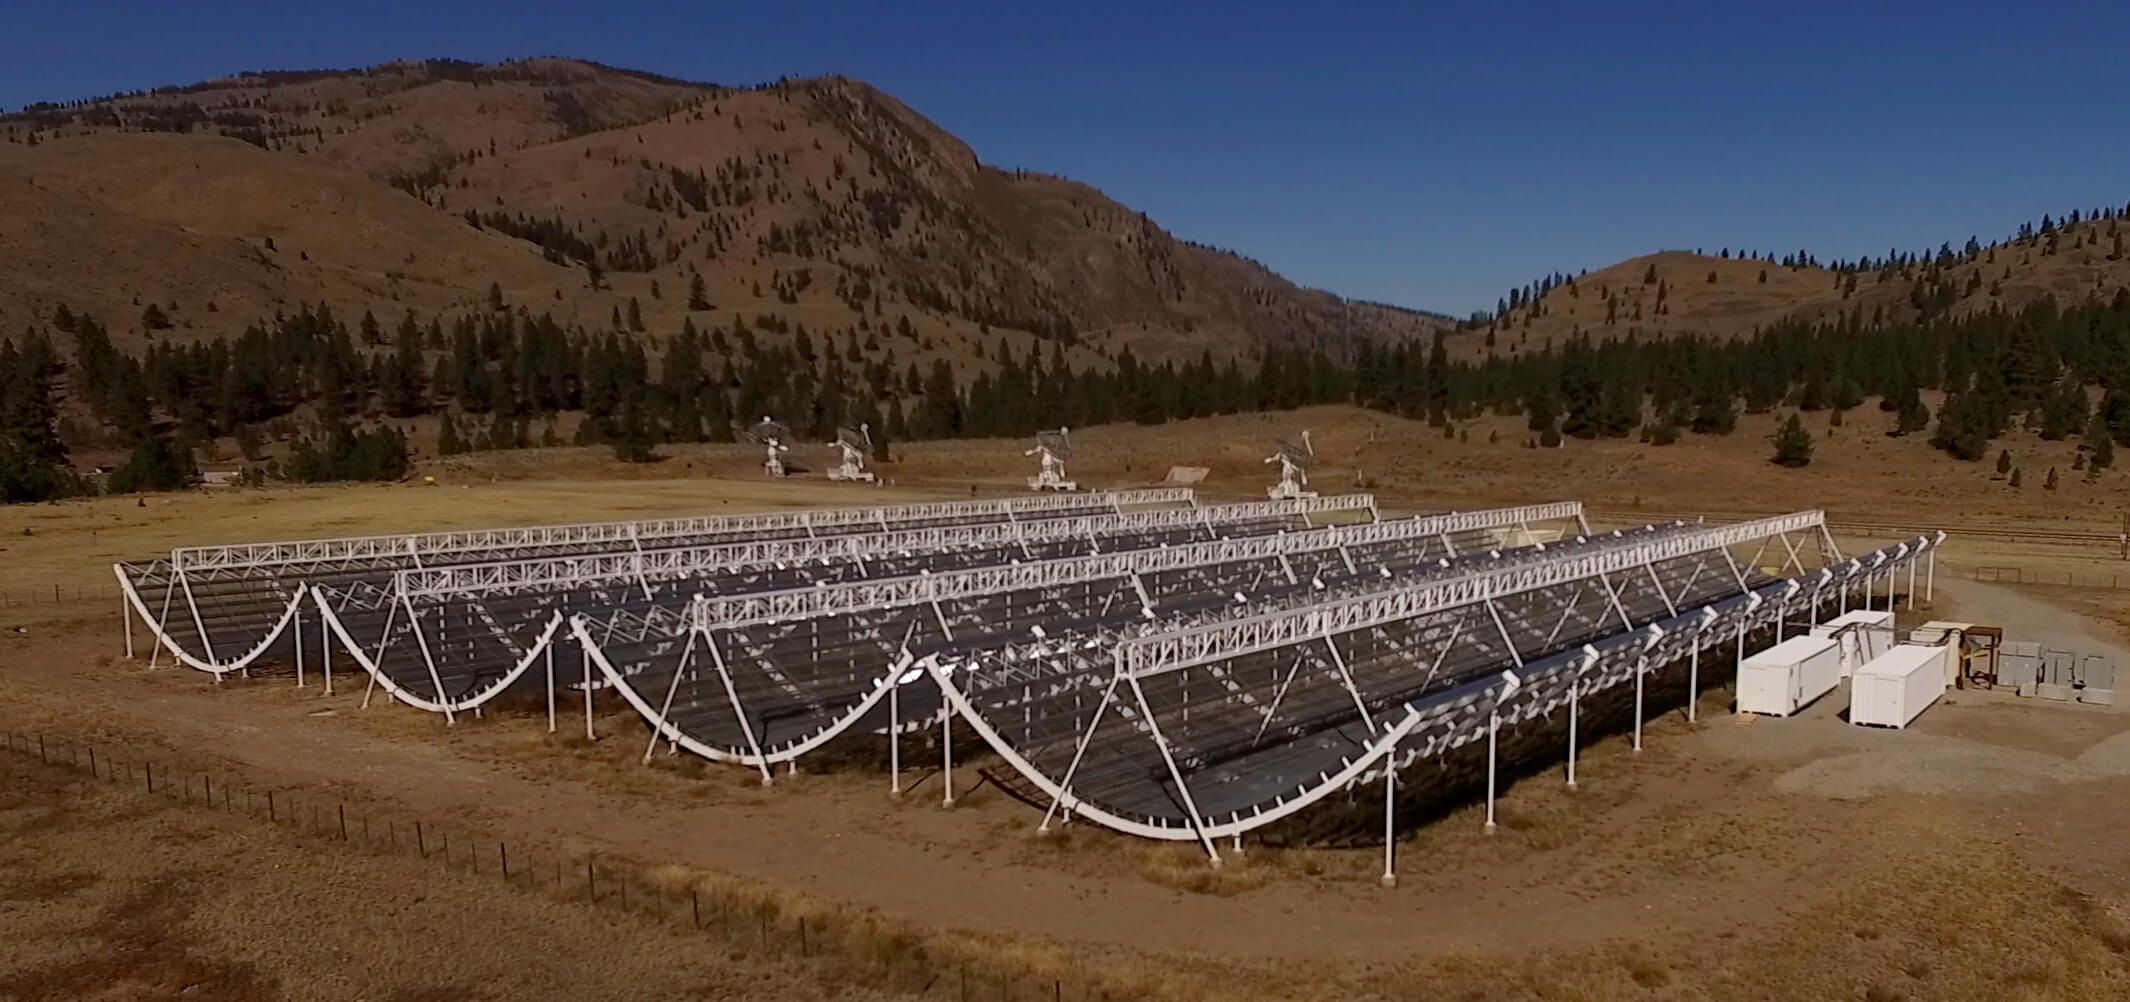
\includegraphics[width=3.2in]{Figures/chime.jpg}
  }


  \frame{
%\vspace{-0.5in}
    \frametitle{Reflections}
    \begin{itemize}
        \item high performance custom codes quickly adaptable to new platforms
        \item 8-bit fixed point rennaisance: N-body, astrophysical
          signal processing, Machine Learning
        \item heterogeneous future: GPU's, FPGAs
    \end{itemize}
\vspace{-0.01in}\hspace{.3in}
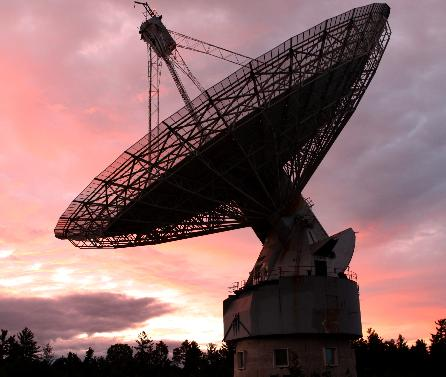
\includegraphics[width=2.2in]{Figures/aro.jpg}
  }


  \frame{
%\vspace{-0.5in}
    \frametitle{Future possibilities}
    \begin{itemize}
        \item excellence in Theoretical Astrophysics: raise
          international visibility, increase total available funding
        \item build on strengths: national bridges, events
        \item new partnerships: industry, foundations
    \end{itemize}
  }



\end{document}
